\section{Design of PCStream}
In this section, we describe in detail the proposed automatic stream management
technique, \textit{PCStream}.  We first explain a mechanism that automatically
obtains the program context (PC) value at runtime, and then describe how
multiple write streams with different PC values are combined and delivered to
an SSD. Finally, we introduce an additional technique that further optimizes
PCStream.

%\subsection{Design overview}

Figure~\ref{fig:architecture} shows the overall architecture of PCStream, which
is composed of a PC extractor, a lifetime analyzer, and a PC-to-stream mapper.
The PC extractor is implemented in the Linux kernel as part of a system call
handler: its responsibility is for intercepting write-related system calls
(e.g., \texttt{write()}, \texttt{writev()}, and so on) and extracting a PC
value.  This enables us to keep track of PC values corresponding to new write
streams from a specific module of an application. An obtained PC value is
forwarded to the lifetime analyzer that estimates expected lifetimes of data
belonging to a given PC. To know when data is deleted or removed, the lifetime
analyzer also intercepts TRIM requests from a file system.  Based on the
lifetime information, the PC-to-stream mapper clusters PC values with similar
lifetimes and maps them together to the same stream ID.  This mapping is
required because, while the number of PCs is unlimited, the number of stream
IDs exposed by an SSD is limited to 8 or 16.

%Figure~\ref{fig:architecture} shows the overall architecture of PCStream.  When
%the write system call handler is called from the user process, it passes the
%user process information to the PC Extractor module.  Then the PC value is
%extracted from the call stack of the writing process by the proposed method
%which will be explained in the following subsection.  In order to analyze the
%lifetime of PCs, we need to maintain the written time and the update/delete
%time of the data for each PC.  The lifetime of data starts when they are
%written for the first time, and ends when they are updated or deleted.  The
%Lifetime Monitor module gets LBAs from the write handler to maintain the
%written time or update time of the data written to the address.  When we get
%TRIM command, the TRIM handler also passes the LBA on to the Lifetime Monitor
%Module for keeping the delete time.  Together with the PC values and their
%lifetimes, we can analyze the lifetime of the PCs of the system.  When the
%number of PCs are greater than the number of streams, we cluster several PCs of
%similar lifetime into a PC group to assign the same stream.  Finally, the
%Stream Allocation module dynamically allocates PC group to the proper stream
%according to the mapping policy.  The detailed mapping policy will be described
%in Section 3.3.

\begin{figure}[t]
	\centering
	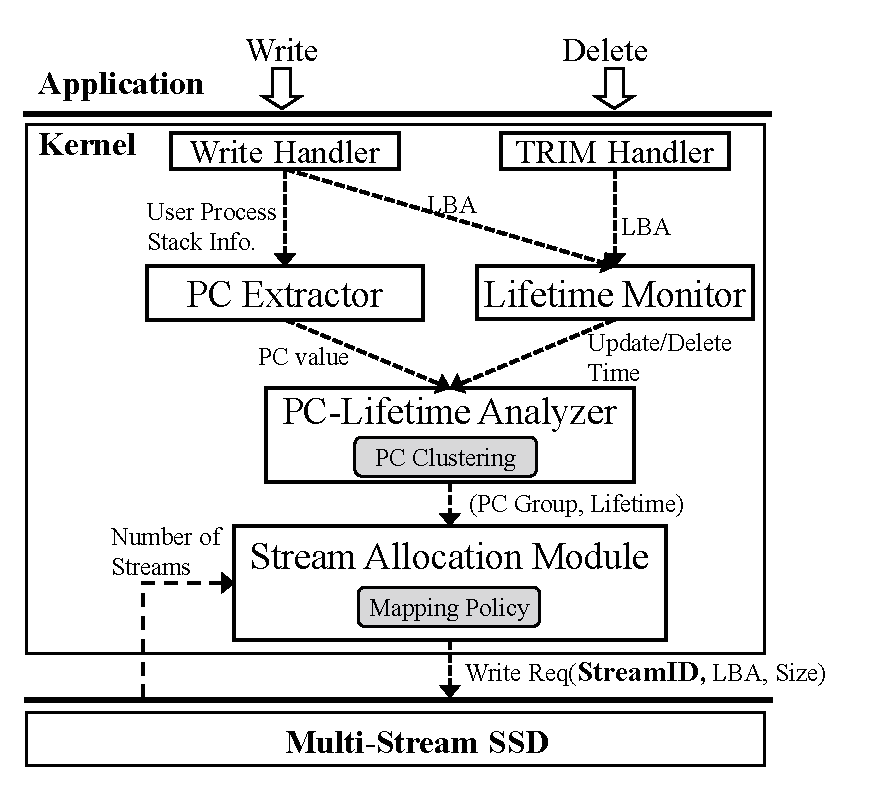
\includegraphics[width=0.8\linewidth]{figure/architecture2}
	\caption{An overall architecture of {\sf PCStream}}
	\label{fig:architecture}
	%\vspace{-20pt}
\end{figure}

\subsection{Automatic PC computation}
As mentioned earlier, a PC value is defined as the sum of the program counter
values along the execution path of the function call.  A function call involves
pushing the next program counter to the process stack as a return address,
which  is used as a return location to keep executing a caller function when a
callee function is finished.  In general, by using a frame register, we are
able to back-track the stack frames of the process and selectively collect
return addresses, which are then used for computing a PC value. For example,
Figure~\ref{fig:getpc}(a) illustrates how a PC value is obtained by
back-tracking the process stack.

Unfortunately, C/C++ compilers (e.g., GNU GCC) often optimize an output code so
that it does not use a frame register when calling functions.  One example is a
{\tt -fomit-frame-pointer} option of GCC. While it is effective in saving
precious resources like CPU registers, this makes it difficult for us to
selectively back-track return addresses only. One alternative is fully examine
every word in the process stack and find out ones that point to the code
segment of the process's virtual address.  Modern OSes divide the process's
virtual address into segments for their purposes, and thus program instructions
(code) are stored in a specific range of the virtual address space (e.g.,
\textcolor{red}{\texttt{0xXXXXh}} to \textcolor{red}{\texttt{0xYYYYh}} in the
Linux).  If there are words that hold a value pointing to somewhere in the code
segment, they are highly likely to be one of the return values.  
\begin{comment} % DO NO REMOVE
Moreover, since the PC extractor is implemented in the kernel, it is not only
able to access the entire virtual address of a process, but also know the
address space layout.
\end{comment}

Searching the entire process stack would require long CPU time. Therefore, the
search process is finished when it finds a certain number of return addresses
in the stack. Currently, this threshold value is set to 5.  In our experiments
with a 3.4 GHz CPU machine, the search process only takes 300-400 $n$sec, so
its overhead is not so huge.  

\begin{figure}[t]
	\centering
	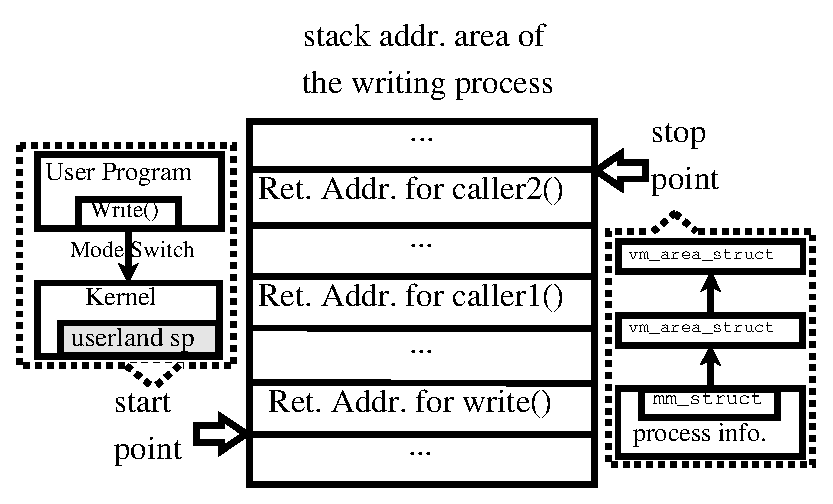
\includegraphics[width=1\linewidth]{figure/getpc}
	\vspace{-10pt}
	\caption{An automatic PC extraction method under compiler optimizations.}
	\label{fig:getpc}
	\vspace{-20pt}
\end{figure}

\subsection{Stream Allocation Policy}
In this paper, we focus on to show the feasibility of the PC-based approach, 
so we limits several factors of PCStream.
The number of application programs is limited to one, 
and we assume the SSD can support enough number of streams
to have 1:1 mapping policy for PCs and streams.
Since every PC is mapped to stream under the 1:1 mapping, 
we do not need to analyze the lifetime of PCs 
or dynamically allocate streams.
The implementation of those modules 
is left as a future work. 

For example, dynamic m:n mapping algorithm is
needed for responding to changes of
the application layer (increased number of PCs)
or the device layer (decreased number of streams).
For the PC clustering, we need to define the lifetime similarity of two PCs
and develop a clustering algorithm.
Also, we will develop the data structure
for the Lifetime Monitor to efficiently find a corresponding PC 
based on the discarded LBA because the deletion does not
make the write program context.

\subsection{Stream Refinement}
According to our observations, the lifetime of data is similar 
for contexts with simple operations such as log, as shown in section 2, 
but some contexts generate various lifetime data.
The compaction behavior of RocksDB belongs to a such context.
Compaction moves the flushed data to the different levels
of the LSM-tree~\cite{RocksDB}, 
so the data generated in one compaction context has 
different life characteristics depending on the target level.
Like RocksDB, LSM-tree-based DBs tend to have a longer 
data lifetime at lower levels~\cite{Level}.
Since the allocated capacity increases as the level goes down, 
the cycle of compaction, which deletes files, is long at low level.
In order to see the difference in the lifetime of each compaction target level,
we modified the RocksDB code to distinguish files according to the compaction level.
Figure~\ref{fig:compaction} shows the lifetime distribution of 
different compaction level data and compaction context data.

\begin{figure}[!t]
\centering
\hspace{1pt}
\subfloat[compaction:L2]{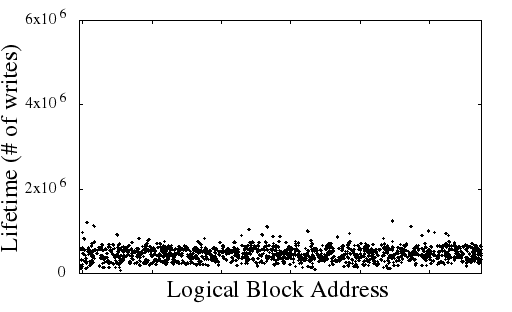
\includegraphics[width=0.23\textwidth]{figure/type_4b}}  % data from 4/03040047
\subfloat[compaction:L3]{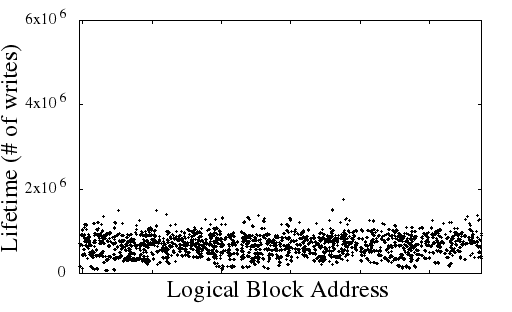
\includegraphics[width=0.23\textwidth]{figure/type_5b}}
\hfill
\vspace{-10pt}
\subfloat[compaction:L4] {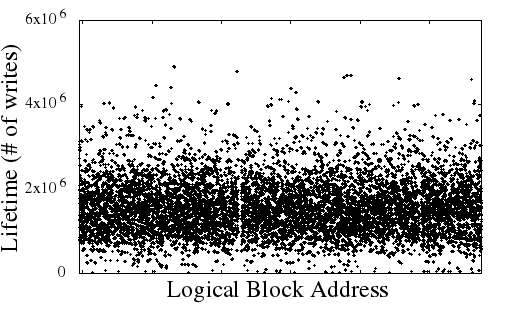
\includegraphics[width=0.23\textwidth]{figure/type_6b}}
\subfloat[PC ID: \#4]{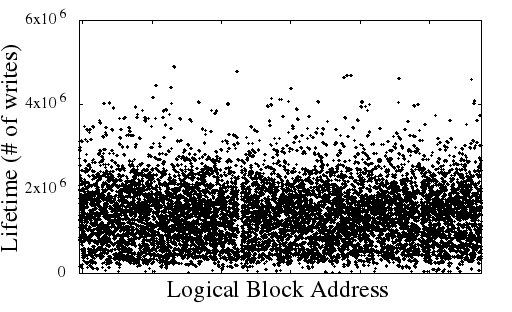
\includegraphics[width=0.23\textwidth]{figure/pc_3b}}
\vspace{-10pt}
\caption{The lifetime distribution of compaction context.} 
\label{fig:compaction}
\vspace{-25pt}
\end{figure}

Level 2 data in Figure~\ref{fig:compaction}(a) and 
level 3 data in Figure~\ref{fig:compaction}(b) seem to have 
a limited lifetime due to the frequent compaction.
On the other hand, because of the long compaction period 
due to the largest space of LSM-tree's lowest level, 
the lifetime is longer than other levels as shown in ~\ref{fig:compaction}(c).
Also, since the target file of the compaction is determined 
by the range of key values of the file~\cite{RocksDB}, 
the previously created file can be deleted 
by participating in the compaction. 
Therefore, the data stored at the lowest level has a very wide lifetime.
However, since all of these data are created in the same context, 
PC 4 can not distinguish any data of the compaction as shown in ~\ref{fig:compaction}(d).
In order to overcome the limitation of PC-based data classification,
we suggest a new optimization technique for multi-stream SSD 
rather than asking application to differentiate the compaction function according to its level.

Basically, the reason for distinguishing data of a similar lifetime is 
to match the timing of data invalidation. 
If long-lived data is gathered together excluding short-lived data, 
there would be no significant impact on WAF. 
So if we store the long-lived data separately even after 
the data is written to the wrong stream, 
we can greatly reduce the side effects of the limitation. 
Therefore, we consider a valid page copied during the GC 
as a misplaced long-lived data 
and allocate a separate substream to accommodate it. 
For example, if a PC with various lifetimes is assigned to stream A, 
we define stream A' as a substream of A and 
move the valid page of stream A to stream A' during GC. 
This prevents long lifetime data of stream A from being repeatedly copied 
by GC.



